\documentclass[a4paper,11pt]{article}
\usepackage{amssymb}
\usepackage[polish]{babel}
\usepackage[utf8]{inputenc}
\usepackage[T1]{fontenc}
\usepackage{array}
\usepackage{graphicx}
\usepackage{anysize}
\usepackage{enumerate}
\usepackage{times}
\usepackage{geometry}
\usepackage{amsthm}
\usepackage{pgfplots}
\usepackage{sidecap}
\usepackage{wrapfig}
\usepackage[format=hang,font=small,labelfont=bf]{caption}
\usepackage[intlimits]{amsmath}
\marginsize{3cm}{3cm}{1.5cm}{1.5cm}
\sloppy

\begin{document}
\begin{flushright}
Załącznik nr 1
\end{flushright}

\begin{center}
\begin{LARGE}
\textbf{Wahadło fizyczne -- wstęp teoretyczny}
\end{LARGE}
\end{center}

\section{Definicje i podstawowe zależności dla wielkości kinetycznych opisujących ruch obrotowy}
\textbf{Ruch obrotowy} bryły sztywnej to taki ruch, w którym wszystkie punkty bryły poruszają się po okręgach o środkach leżących na jednej prostej zwanej osią obrotu.  
\subsection{Położenie kątowe}
Położeniem kątowym ciała $\theta$ nazywamy kąt, jaki tworzy linia odniesienia z pewnym stałym kierunkiem. Jeśli ten kąt wyrażony jest w mierze łukowe (radianach), to:
$$\theta = \frac{s}{r},$$
gdzie $s$ jest długością odpowiadającą kątowi $\theta$ łuku okręgu o promieniu $r$. 
\subsection{Przemieszczenie kątowe}
Jeśli ciało obracające się wokół osi zmienia swoje położenie kątowe z $\theta_{1}$ na $\theta_{2}$, to doznaje ono przemieszczenia kątowego:
$$\Delta \theta = \theta_{2} - \theta_{1}.$$
Jeśli obrót odbywa się w kierunku przeciwnym do kierunku ruchu wskazówek zegara, to $\delta \theta$ jest dodatnie, a ujemne, jeśli obrót odbywa się w kierunku zgodnym z kierunkiem ruchu wskazówek zegara.
\subsection{Prędkość kątowa}
Jeśli ciała doznaje przemieszczenia kątowego $\delta \theta$ w przedziale czasu  $\Delta t$, to jego średnia prędkość kątowa wynosi:
$$\omega_{sr} = \dfrac{\Delta \theta}{\Delta t},$$
a prędkość chwilowa tego ciała jest równa:
$$\omega_{sr} = \dfrac{d\theta}{dt}.$$
Obie te wielkości $\omega_{sr}$ i $\omega$ są wektorami, których kierunek wyznacza się regułą prawej dłoni.
\subsection{Przyspieszenie kątowe}
Jeśli prędkość kątowa ciała zmienia się z $\omega_{1}$ na $\omega_{2}$ w przedziale czasu $\Delta t = t{2} - \theta_{1}$, to średnie przyspieszenie kątowe wynosi:
$$\epsilon_{sr} = \dfrac{\Delta \omega}{\Delta t},$$
a przyspieszenie kątowe chwilowe jest równe:
$$\epsilon = \dfrac{d\omega}{dt}.$$

\subsection{Jednostajny i niejednostajny ruch obrotowy}
\textbf{Ruch obrotowy jednostajny} to ruch obrotowy ze stałą prędkością kątową $\omega = \frac{2\pi}{T}$.
\textbf{Ruch obrotowy niejednostajny} to ruch po torze o kształcie okręgu ze zmienną wartością prędkości. W~zależności od charakteru tej zmiany, można wyróżnić \textbf{ruch jednostajnie zmienny po okręgu} (wartość przyspieszenia kątowego jest stała) oraz \textbf{ruch niejednostajnie zmienny po okręgu} – wartość przyspieszenia kątowego opisana jest funkcją w czasie.


\section{Definicje i podstawowe zależności dla wielkości dynamicznych opisujących ruch obrotowy.}

\subsection{Moment bezwładności}
Moment bezwładności to miara bezwładności ciała w ruchu obrotowym względem ustalonej osi obrotu. Im większy moment, tym trudniej zmienić ruch obrotowy ciała.

\subsection{Moment pędu} 
Moment pędu punktu materialnego o pędzie $\vec{p}$, którego położenie opisane jest wektorem wodzącym $\vec{r}$ względem danego układu odniesienia definiuje się jako wektor będący rezultatem iloczynu wektorowego wektora położenia i pędu:
$$\vec{L}=\vec{r} \times \vec{p}.$$
Z własności iloczynu wektorowego wynika, że wartość bezwzględna momentu pędu jest równa  
$$L=|r|\cdot |p| \cdot sin\theta,$$ 
gdzie $\theta$ oznacza kąt między wektorami $\vec{r}$ i $\vec{p}$. Dla ciała o momencie bezwładności $I$ obracającego się wokół ustalonej osi z prędkością kątową $\omega$ moment pędu można wyrazić wzorem  
$$L=I\cdot \omega.$$

\subsection{Moment siły} 
Moment siły $\vec{F}$ względem punktu $O$ to iloczyn wektorowy promienia wodzącego $\vec{r}$, o początku w punkcie $O$ i końcu w punkcie przyłożenia siły, oraz siły $\vec{F}$:  
$$\vec{M}=\vec{r} \times \vec{F},$$ 
co możemy zapisać jako:  
$$M=m\cdot g\cdot a\cdot sin\theta,$$ 
gdzie $a$ jest odległością środka masy $S$ od osi obrotu, a $\theta$ odchyleniem od pionu.
\subsection{Druga zasada dynamiki dla ruchu obrotowego}
Jeśli na pewne ciało, o momencie bezwładności względem tej osi równym I, działają zewnętrzne siły, które wywierają na to ciało wypadkowy moment siły M, to w wyniku tego ciało będzie obracać się z przyspieszeniem kątowym takim, że: 
$$\vec{M}=I \cdot \vec{\epsilon}.$$

\section{Definicja momentu bezwładności. Wyprowadzenie momentu bezwładności dla jednorodnego pręta o długości $l$ i masie $m$ względem osi prostopadłej do pręta i przechodzącej przez jego środek masy.}
Dla układu oddzielnych cząstek moment bezwładności ciała zdefiniowany jest jako:
$$I=\sum m_{i}r_{i}^{2},$$
a dla ciała o ciągłym rozkładzie masy jako:
$$I=\int r^{2}dm,$$
gdzie wielkości $r$ i $r_{i}$ są odległościami elementów ciała od osi obrotu.
$$$$
Pręt to walec o promieniu zbiegającym do zera, więc można go traktować jako figurę jednowymiarową. Gęstość liniowa pręta to $\lambda = \frac{m}{l}$, wobec tego $dm = \lambda dx = \frac{m}{l} dx$. Moment bezwładności takiego elementu pręta to $dI = \frac{m}{l} x^2 dx$. Środek układu współrzędnych pokrywa się ze środkiem masy pręta, co daje nam: 
$$I = \frac{m}{l} \int_{-\frac{l}{2}}^{\frac{l}{2}} x^2 dx = \frac{m}{l} \left( \frac{l^3}{24} + \frac{l^3}{24}\right) = \frac{1}{12} ml^2$$

\section{Twierdzenie Steinera dla momentu bezwładności i przykłady jego zastosowania.}
Twierdzenie to mówi, że jeśli znamy moment bezwładności $I_{S}$ danego ciała względem pewnej osi przechodzącej przez środek masy tego ciała, to aby obliczyć moment bezwładności $I_{0}$ względem dowolnej innej osi równoległej do niej, należy do momentu $I_{S}$ dodać iloczyn masy ciała i kwadratu odległości $a$ między tymi osiami:
$$I_{0}=I_{S}+ma^{2}$$
Na przykład znając moment bezwładności kuli względem osi przechodzącej przez środek jej masy $I_{S}=\dfrac{2}{5}mR^{2}$, możemy wyliczyć moment bezwładności kuli względem osi stycznej do tej kuli:
$$I_{0}=I_{S}+ma^{2}=\dfrac{2}{5}mR^{2}+mR^{2}=\dfrac{7}{5}mR^{2}$$

\section{Ruch harmoniczny, równanie ruchu i parametry opisujące ruch.}

Ruch harmoniczny -- drgania opisane funkcją sinusoidalną (harmoniczną). Jest to najprostszy w~opisie matematycznym rodzaj drgań. Z prawa Hook'a mamy:
$$\vec{F}=-k\vec{x},$$
gdzie $F$ to siła, $k$ to współczynnik sprężystości, a $x$ to wychylenie z położenia równowagi.
Stosując drugą zasadę dynamiki Newtona ($F = ma$) i rozwiązując równanie różniczkowe drugiego stopnie otrzymujemy równanie ruchu harmonicznego: 
$$x(t)=Asin(\omega t +\varphi),$$
gdzie $\omega=\sqrt{\dfrac{k}{m}}$ to częstość kołowa drgań, $A$ to amplituda (wychylenie maksymalne), $\varphi$ to faza początkowa ruchu, a cały argument funkcji sinus to faza ruchu.
Czas wykonania jednego pełnego drgania to okres i wynosi $T=\dfrac{2\pi}{\omega}$, a ilość drgań wykonanych w określonej jednostce czasu
to częstotliwość $\nu=\dfrac{\omega}{2\pi}[Hz]$.

\section{Wahadło matematyczne. Opis ruchu wahadła matematycznego dla małych drgań. Okres drgań tego wahadła.}
\begin{wrapfigure}{l}{0.4\textwidth}
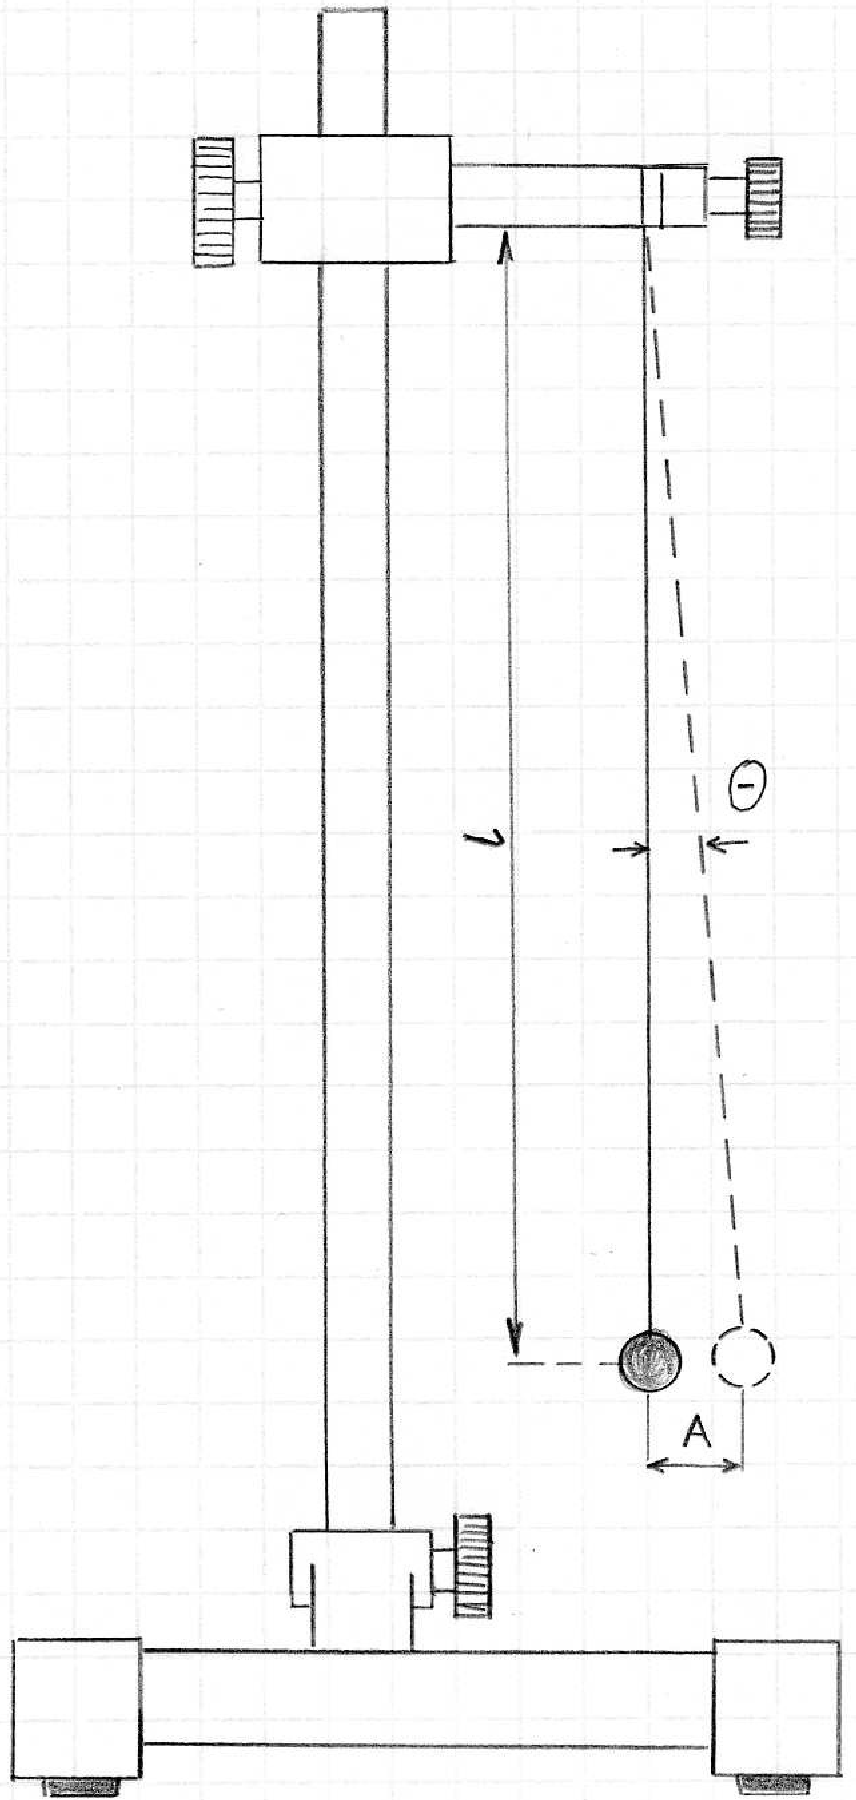
\includegraphics[width=0.4\textwidth]{./wahadlomat}
\caption{Wahadło matematyczne}
\end{wrapfigure}
Wahadło matematyczne to ciało o masie punktowej zawieszone na cienkiej, nierozciągliwej nici. Kiedy ciało wytrącimy z równowagi, zaczyna się ono wahać w płaszczyźnie pionowej pod wpływem siły ciężkości ruchem okresowym.
Aby wyprowadzić wzór na okres zapisujemy drugą zasadę dynamiki dla wahadła:
$$ml^{2} \frac{d^{2} \theta }{dt^{2}}=-mgl\sin \theta.$$
Stosując przybliżenie małych kątów $\sin \theta \approx \theta$ otrzymujemy:
$$\frac{d^{2} \theta }{dt^{2}}=- \frac{g}{l} \theta.$$
Mamy równanie różniczkowe drugiego rzędu, z którego otrzymujemy:
$$\theta =A\sin (\omega t + \varphi)$$ 
gdzie $\omega = \sqrt{ \dfrac{g}{l} }$ to częstość kołowa drgań, $A$ to amplituda (wychylenie maksymalne), $\varphi$ to faza początkowa ruchu, a cały argument funkcji sinus to faza ruchu.
Aby wyliczyć okres wahadła dokonujemy podstawienia:
$$\frac{2\pi}{T}= \sqrt{\frac{g}{l}}$$
$$T=2\pi\sqrt{\dfrac{l}{g}}$$
$$$$
\section{Wahadło fizyczne. Przybliżony opis ruchu wahadła fizycznego za pomocą równania ruchu harmonicznego. Okres drgań wahadła fizycznego w przybliżeniu harmonicznym.} 

Wahadło fizyczne to bryła sztywna mogąca poruszać się swobodnie względem osi obrotu $O$ nie przechodzącej przez środek ciężkości tej bryły $S$. W~polu grawitacyjnym wahadło fizyczne wykonuje ruch drgający -- jest to ruch obrotowy względem poziomej osi przechodzącej przez punkt $O$. Przyczyną tego ruchu jest moment siły ciężkości prostopadły do płaszczyzny poniższego rysunku.
 
\begin{wrapfigure}{r}{0.38\textwidth}
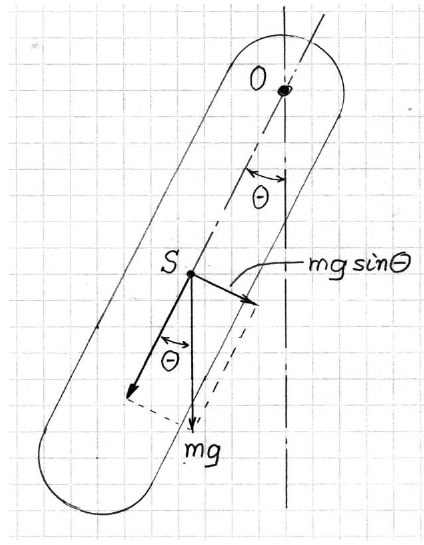
\includegraphics[width=0.38\textwidth]{./wahadlo}
\caption{Wahadło fizyczne}
\end{wrapfigure}
\noindent Zgodnie z \textbf{drugą zasadą dynamiki dla ruchu obrotowego} ruch ten opisuje równanie:
$$ I_{o}\displaystyle \frac{d^{2}\theta}{dt^{2}}=-mga\sin\theta,$$   
gdzie:

$I_{o}$ -- moment bezwładności bryły względem osi obrotu,

$\theta$ -- kąt wychylenia od położenia równowagi,

$t$ -- czas,

$m$ -- masa bryły,

$g$ -- przyspieszenie ziemskie,

$a$ -- odległość osi obrotu od środka ciężkości.

\noindent Równanie to opisuje ruch drgający, który nie jest ruchem harmonicznym. Zakładając, że amplituda drgań (kąt maksymalnego wychylenia) nie przekracza kilku stopni, możemy skorzystać z~przybliżenia:

$$\displaystyle \sin\theta\approx\theta=\frac{x}{a},$$
gdzie $x$ to długość łuku wychylenia środka ciężkości z położenia równowagi. Wstawiając taką zależność do powyższego równania otrzymujemy:
$$\displaystyle \frac{d^{2}x}{dt^{2}}=-\frac{mga}{I_{o}}x,$$
jest to równanie ruchu harmonicznego z okresem:
$$T=2\pi\sqrt{\frac{I_{o}}{mga}}$$

\end{document}
